 %% History:
% Pavel Tvrdik (26.12.2004)
%  + initial version for PhD Report
%
% Daniel Sykora (27.01.2005)
%
% Michal Valenta (3.12.2008)
% rada zmen ve formatovani (diky M. Duškovi, J. Holubovi a J. Žďárkovi)
% sjednoceni zdrojoveho kodu pro anglickou, ceskou, bakalarskou a diplomovou praci

% One-page layout: (proof-)reading on display
%%%% \documentclass[11pt,oneside,a4paper]{book}
% Two-page layout: final printing
\documentclass[11pt,twoside,a4paper]{book}   
%=-=-=-=-=-=-=-=-=-=-=-=--=%
% The user of this template may find useful to have an alternative to these 
% officially suggested packages:
\usepackage[czech, english]{babel}
\usepackage[T1]{fontenc} % pouzije EC fonty 
% pripadne pisete-li cesky, pak lze zkusit take:
% \usepackage[OT1]{fontenc} 
\usepackage[utf8]{inputenc}
%=-=-=-=-=-=-=-=-=-=-=-=--=%
% In case of problems with PDF fonts, one may try to uncomment this line:
%\usepackage{lmodern}
%=-=-=-=-=-=-=-=-=-=-=-=--=%
%=-=-=-=-=-=-=-=-=-=-=-=--=%
% Depending on your particular TeX distribution and version of conversion tools 
% (dvips/dvipdf/ps2pdf), some (advanced | desperate) users may prefer to use 
% different settings.
% Please uncomment the following style and use your CSLaTeX (cslatex/pdfcslatex) 
% to process your work. Note however, this file is in UTF-8 and a conversion to 
% your native encoding may be required. Some settings below depend on babel 
% macros and should also be modified. See \selectlanguage \iflanguage.
%\usepackage{czech}  %%%%%\usepackage[T1]{czech} %%%%[IL2] [T1] [OT1]
%=-=-=-=-=-=-=-=-=-=-=-=--=%

%%%%%%%%%%%%%%%%%%%%%%%%%%%%%%%%%%%%%%%
% Styles required in your work follow %
%%%%%%%%%%%%%%%%%%%%%%%%%%%%%%%%%%%%%%%
\usepackage{graphicx}
%\usepackage{indentfirst} %1. odstavec jako v cestine.

\usepackage{listings}
\usepackage{color}

\definecolor{dkgreen}{rgb}{0,0.6,0}
\definecolor{gray}{rgb}{0.5,0.5,0.5}
\definecolor{mauve}{rgb}{0.58,0,0.82}
 
\lstset{ %
  language=Ruby,                % the language of the code
  basicstyle=\small,           % the size of the fonts that are used for the code
  numbers=left,                   % where to put the line-numbers
  numberstyle=\scriptsize\color{gray},  % the style that is used for the line-numbers
%  stepnumber=2,                   % the step between two line-numbers. If it's 1, each line 
                                  % will be numbered
  numbersep=5pt,                  % how far the line-numbers are from the code
  backgroundcolor=\color{white},      % choose the background color. You must add \usepackage{color}
  showspaces=false,               % show spaces adding particular underscores
  showstringspaces=false,         % underline spaces within strings
  showtabs=false,                 % show tabs within strings adding particular underscores
  frame=single,                   % adds a frame around the code
  rulecolor=\color{black},        % if not set, the frame-color may be changed on line-breaks within not-black text (e.g. commens (green here))
  tabsize=2,                      % sets default tabsize to 2 spaces
  captionpos=b,                   % sets the caption-position to bottom
  breaklines=true,                % sets automatic line breaking
  breakatwhitespace=false,        % sets if automatic breaks should only happen at whitespace
  title=\lstname,                   % show the filename of files included with \lstinputlisting;
                                  % also try caption instead of title
  keywordstyle=\color{blue},          % keyword style
  commentstyle=\color{dkgreen},       % comment style
  stringstyle=\color{mauve},         % string literal style
 %escapeinside={\%*}{*)},            % if you want to add a comment within your code
  morekeywords={*,...}               % if you want to add more keywords to the set
}


\usepackage{k336_thesis_macros} % specialni makra pro formatovani DP a BP
 % muzete si vytvorit i sva vlastni v souboru k336_thesis_macros.sty
 % najdete  radu jednoduchych definic, ktere zde ani nejsou pouzity
 % napriklad: 
 % \newcommand{\bfig}{\begin{figure}\begin{center}}
 % \newcommand{\efig}{\end{center}\end{figure}}
 % umoznuje pouzit prikaz \bfig namisto \begin{figure}\begin{center} atd.


%%%%%%%%%%%%%%%%%%%%%%%%%%%%%%%%%%%%%
% Zvolte jednu z moznosti 
% Choose one of the following options
%%%%%%%%%%%%%%%%%%%%%%%%%%%%%%%%%%%%%
%\newcommand\TypeOfWork{Diplomová práce} \typeout{Diplomova prace}
% \newcommand\TypeOfWork{Master's Thesis}   \typeout{Master's Thesis} 
\newcommand\TypeOfWork{Bakalářská práce}  \typeout{Bakalarska prace}
% \newcommand\TypeOfWork{Bachelor's Project}  \typeout{Bachelor's Project}


%%%%%%%%%%%%%%%%%%%%%%%%%%%%%%%%%%%%%
% Zvolte jednu z moznosti 
% Choose one of the following options
%%%%%%%%%%%%%%%%%%%%%%%%%%%%%%%%%%%%%
% nabidky jsou z: http://www.fel.cvut.cz/cz/education/bk/prehled.html

%\newcommand\StudProgram{Elektrotechnika a informatika, dobíhající, Bakalářský}
%\newcommand\StudProgram{Elektrotechnika a informatika, dobíhající, Magisterský}
% \newcommand\StudProgram{Elektrotechnika a informatika, strukturovaný, Bakalářský}
% \newcommand\StudProgram{Elektrotechnika a informatika, strukturovaný, Navazující magisterský}
\newcommand\StudProgram{Softwarové technologie a management, Bakalářský}
% English study:
% \newcommand\StudProgram{Electrical Engineering and Information Technology}  % bachelor programe
% \newcommand\StudProgram{Electrical Engineering and Information Technology}  %master program


%%%%%%%%%%%%%%%%%%%%%%%%%%%%%%%%%%%%%
% Zvolte jednu z moznosti 
% Choose one of the following options
%%%%%%%%%%%%%%%%%%%%%%%%%%%%%%%%%%%%%
% nabidky jsou z: http://www.fel.cvut.cz/cz/education/bk/prehled.html

%\newcommand\StudBranch{Výpočetní technika}   % pro program EaI bak. (dobihajici i strukt.)
%\newcommand\StudBranch{Výpočetní technika}   % pro prgoram EaI mag. (dobihajici i strukt.)
\newcommand\StudBranch{Softwarové inženýrství}            %pro STM
%\newcommand\StudBranch{Web a multimedia}                  % pro STM
%\newcommand\StudBranch{Computer Engineering}              % bachelor programe
%\newcommand\StudBranch{Computer Science and Engineering}  % master programe


%%%%%%%%%%%%%%%%%%%%%%%%%%%%%%%%%%%%%%%%%%%%
% Vyplnte nazev prace, autora a vedouciho
% Set up Work Title, Author and Supervisor
%%%%%%%%%%%%%%%%%%%%%%%%%%%%%%%%%%%%%%%%%%%%

\newcommand\WorkTitle{Ruby - Access Control List}
\newcommand\FirstandFamilyName{Jan Širl}
\newcommand\Supervisor{Ing. Pavel Strnad}


% Pouzijete-li pdflatex, tak je prijemne, kdyz bude mit vase prace
% funkcni odkazy i v pdf formatu
\usepackage[
pdftitle={\WorkTitle},
pdfauthor={\FirstandFamilyName},
bookmarks=true,
colorlinks=true,
breaklinks=true,
urlcolor=red,
citecolor=blue,
linkcolor=blue,
unicode=true,
]
{hyperref}



% Extension posted by Petr Dlouhy in order for better sources reference (\cite{} command) especially in Czech.
% April 2010
% See comment over \thebibliography command for details.

\usepackage[square, numbers]{natbib}             % sazba pouzite literatury
%\usepackage{url}
%\DeclareUrlCommand\url{\def\UrlLeft{<}\def\UrlRight{>}\urlstyle{tt}}  %rm/sf/tt
%\renewcommand{\emph}[1]{\textsl{#1}}    % melo by byt kurziva nebo sklonene,
\let\oldUrl\url
\renewcommand\url[1]{<\texttt{\oldUrl{#1}}>}




\begin{document}

%%%%%%%%%%%%%%%%%%%%%%%%%%%%%%%%%%%%%
% Zvolte jednu z moznosti 
% Choose one of the following options
%%%%%%%%%%%%%%%%%%%%%%%%%%%%%%%%%%%%%
\selectlanguage{czech}
%\selectlanguage{english} 

% prikaz \typeout vypise vyse uvedena nastaveni v prikazovem okne
% pro pohodlne ladeni prace


\iflanguage{czech}{
	 \typeout{************************************************}
	 \typeout{Zvoleny jazyk: cestina}
	 \typeout{Typ prace: \TypeOfWork}
	 \typeout{Studijni program: \StudProgram}
	 \typeout{Obor: \StudBranch}
	 \typeout{Jmeno: \FirstandFamilyName}
	 \typeout{Nazev prace: \WorkTitle}
	 \typeout{Vedouci prace: \Supervisor}
	 \typeout{***************************************************}
	 \newcommand\Department{Katedra počítačů}
	 \newcommand\Faculty{Fakulta elektrotechnická}
	 \newcommand\University{České vysoké učení technické v Praze}
	 \newcommand\labelSupervisor{Vedoucí práce}
	 \newcommand\labelStudProgram{Studijní program}
	 \newcommand\labelStudBranch{Obor}
}{
	 \typeout{************************************************}
	 \typeout{Language: english}
	 \typeout{Type of Work: \TypeOfWork}
	 \typeout{Study Program: \StudProgram}
	 \typeout{Study Branch: \StudBranch}
	 \typeout{Author: \FirstandFamilyName}
	 \typeout{Title: \WorkTitle}
	 \typeout{Supervisor: \Supervisor}
	 \typeout{***************************************************}
	 \newcommand\Department{Department of Computer Science and Engineering}
	 \newcommand\Faculty{Faculty of Electrical Engineering}
	 \newcommand\University{Czech Technical University in Prague}
	 \newcommand\labelSupervisor{Supervisor}
	 \newcommand\labelStudProgram{Study Programme} 
	 \newcommand\labelStudBranch{Field of Study}
}




%%%%%%%%%%%%%%%%%%%%%%%%%%    Poznamky ke kompletaci prace
% Nasledujici pasaz uzavrenou v {} ve sve praci samozrejme 
% zakomentujte nebo odstrante. 
% Ve vysledne svazane praci bude nahrazena skutecnym 
% oficialnim zadanim vasi prace.
{
\pagenumbering{roman} \cleardoublepage \thispagestyle{empty}
\chapter*{Na tomto místě bude oficiální zadání vaší práce}
\begin{itemize}
\item Toto zadání je podepsané děkanem a vedoucím katedry,
\item musíte si ho vyzvednout na studiijním oddělení Katedry počítačů na Karlově náměstí,
\item v jedné odevzdané práci bude originál tohoto zadání (originál zůstává po obhajobě na katedře),
\item ve druhé bude na stejném místě neověřená kopie tohoto dokumentu (tato se vám vrátí po obhajobě).
\end{itemize}
\newpage
}

%%%%%%%%%%%%%%%%%%%%%%%%%%    Titulni stranka / Title page 

\coverpagestarts

%%%%%%%%%%%%%%%%%%%%%%%%%%%    Podekovani / Acknowledgements 

\acknowledgements
\noindent
Chtěl bych především poděkovat panu Ing. Pavlu Strnadovi, že se mě ujal jako vedoucí jak semestrálního projektu tak Bakalářské práce a poskytl mi rady a motivaci. Poděkování také patří mé přítelkyni a rodině za nemalou podporu při tvorbě bakalářské práce a v průběhu celého studia.

%%%%%%%%%%%%%%%%%%%%%%%%%%%   Prohlaseni / Declaration 

\declaration{V~Praze dne 25.\,5.\,2012}
%\declaration{In Prague on March 18, 2012}


%%%%%%%%%%%%%%%%%%%%%%%%%%%%    Abstract 
 
\abstractpage
This paper presents the design and implementation of library management access rights in the programming language Ruby.

The library is designed for object XML database and is solved using the Access Control List. Library used for storing and querying the database itself, which communicates with the protocol for remote procedure call and for quering uses current query languages.
The functionality of the library was developed and tested on eXist-db.

% Prace v cestine musi krome abstraktu v anglictine obsahovat i
% abstrakt v cestine.
\vglue60mm

\noindent{\Huge \textbf{Abstrakt}}
\vskip 2.75\baselineskip

\noindent
Tato práce prezentuje návrh a realizaci knihovny pro správu přístupových práv v programovacím jazyku Ruby. 

Knihovna  je určena pro objektovou XML databázi a je řešena pomocí Access Control Listu. Knihovna využívá pro ukládání a dotazování samotnou databázi, se kterou komunikuje pomocí protokolu pro vzdálené volání procedur a pro dotazování používá aktuální dotazovací jazyky. 
Funkčnost knihovny byla vyvíjena a testována pomocí databáze eXist-db.


\noindent
%Očekávají se cca 1 -- 2 odstavce, maximálně půl stránky.

%Abstract
%



%%%%%%%%%%%%%%%%%%%%%%%%%%%%%%%%  Obsah / Table of Contents 

\tableofcontents


%%%%%%%%%%%%%%%%%%%%%%%%%%%%%%%  Seznam obrazku / List of Figures 

\listoffigures


%%%%%%%%%%%%%%%%%%%%%%%%%%%%%%%  Seznam tabulek / List of Tables

\listoftables


%**************************************************************

\mainbodystarts
% horizontalní mezera mezi dvema odstavci
%\parskip=5pt
%11.12.2008 parskip + tolerance
\normalfont
\parskip=0.2\baselineskip plus 0.2\baselineskip minus 0.1\baselineskip

% Odsazeni prvniho radku odstavce resi class book (neaplikuje se na prvni 
% odstavce kapitol, sekci, podsekci atd.) Viz usepackage{indentfirst}.
% Chcete-li selektivne zamezit odsazeni 1. radku nektereho odstavce,
% pouzijte prikaz \noindent.

%**************************************************************

% Pro snadnejsi praci s vetsimi texty je rozumne tyto rozdelit
% do samostatnych souboru nejlepe dle kapitol a tyto potom vkladat
% pomoci prikazu \include{jmeno_souboru.tex} nebo \include{jmeno_souboru}.
% Napr.:
% \chapter{Úvod}

\section{Úvod do problematiky}

Tato bakalářská práce navazuje na můj semestrální projekt. Zabývá se správou - administrací řízení přístupu, jakožto procesu autorizování uživatelů, skupin a počítačů pro přístup k objektům. Tento proces pracuje s pojmy: oprávnění, uživatelská práva a audit objektů. Tato jednotlivá přiřazená oprávnění začleňuje jako položky řízení přístupu (ACE\footnote{Access Control Entry}) a jejich celé sady začleňuje do seznamu přístupových práv (ACL\footnote{Access Control List}). Úkolem bakalářské práce bylo vytvořit, navrhnout a realizovat v jazyce Ruby model uživatelských přístupových práv určený pro objektovou XML\footnote{Extensible Markup Language} databázi.

Součástí práce byl návrh knihovny. Navržená knihovna realizuje správu řízení přístupu pomocí ACL. Knihovnu nazývám Ruby-ACL. Protože moje bakalářská práce je prací implementační, včetně testů navržené knihovny, zaměřil jsem se na specifikaci rozhraní knihovny a na příklady jejího použití. Výsledkem je nejen samotná realizace knihovny, ale i podrobná programátorská dokumentace.

Je-li potřeba zabezpečit zdroje a jeho prostředky, je nutné vzít v úvahu, jakými právy budou disponovat ti, kteří k nim budou přistupovat. Zabezpečit objekt, například dokument či kolekci, lze přidělením oprávnění, která umožňují uživatelům nebo skupinám provádět u tohoto objektu určité akce. Řízení přístupů je činnost zabývající se přidáváním a zamítáním oprávnění přistupujícím.

Ruby je objektově orientovaný, interpretovaný skriptovací programovací jazyk. Díky své jednoduché syntaxi je poměrně snadný, přesto však dostatečně výkonný, aby dokázal konkurovat známějším jazykům jako je Python a Perl. Převzato a upraveno z wikipedie\cite{wiki:Ruby}

ACL je seznam pro řízení přístupů. Seznam určuje, kdo nebo co má povolení přistupovat k objektu a jaké operace s ním může nebo nesmí provádět. V typickém ACL specifikuje každý záznam v seznamu uživatele a operaci\cite{wiki:acl}.

%-------------------------------

\section{Motivace}
Zaujala mě problematika práv, databází a pro mě neznámého jazyka Ruby.
Jádro celé mé motivace, bylo projít si vývojem softwaru, v tomto případě knihovny, od návrhu přes implementaci k testování a dokumentaci a ověřit si získané poznatky z předmětu softwarového inženýrství. Soustředil jsem se na vlastní nápady. Nechtěl jsem skládat a kopírovat polotvary a "lepit" je dohromady.
% \include{2_teorie}

% atd...

%*****************************************************************************
% Úvod
\chapter{Úvod}

\section{Úvod do problematiky}

Tato bakalářská práce navazuje na můj semestrální projekt. Zabývá se správou - administrací řízení přístupu, jakožto procesu autorizování uživatelů, skupin a počítačů pro přístup k objektům. Tento proces pracuje s pojmy: oprávnění, uživatelská práva a audit objektů. Tato jednotlivá přiřazená oprávnění začleňuje jako položky řízení přístupu (ACE\footnote{Access Control Entry}) a jejich celé sady začleňuje do seznamu přístupových práv (ACL\footnote{Access Control List}). Úkolem bakalářské práce bylo vytvořit, navrhnout a realizovat v jazyce Ruby model uživatelských přístupových práv určený pro objektovou XML\footnote{Extensible Markup Language} databázi.

Součástí práce byl návrh knihovny. Navržená knihovna realizuje správu řízení přístupu pomocí ACL. Knihovnu nazývám Ruby-ACL. Protože moje bakalářská práce je prací implementační, včetně testů navržené knihovny, zaměřil jsem se na specifikaci rozhraní knihovny a na příklady jejího použití. Výsledkem je nejen samotná realizace knihovny, ale i podrobná programátorská dokumentace.

Je-li potřeba zabezpečit zdroje a jeho prostředky, je nutné vzít v úvahu, jakými právy budou disponovat ti, kteří k nim budou přistupovat. Zabezpečit objekt, například dokument či kolekci, lze přidělením oprávnění, která umožňují uživatelům nebo skupinám provádět u tohoto objektu určité akce. Řízení přístupů je činnost zabývající se přidáváním a zamítáním oprávnění přistupujícím.

Ruby je objektově orientovaný, interpretovaný skriptovací programovací jazyk. Díky své jednoduché syntaxi je poměrně snadný, přesto však dostatečně výkonný, aby dokázal konkurovat známějším jazykům jako je Python a Perl. Převzato a upraveno z wikipedie\cite{wiki:Ruby}

ACL je seznam pro řízení přístupů. Seznam určuje, kdo nebo co má povolení přistupovat k objektu a jaké operace s ním může nebo nesmí provádět. V typickém ACL specifikuje každý záznam v seznamu uživatele a operaci\cite{wiki:acl}.

%-------------------------------

\section{Motivace}
Zaujala mě problematika práv, databází a pro mě neznámého jazyka Ruby.
Jádro celé mé motivace, bylo projít si vývojem softwaru, v tomto případě knihovny, od návrhu přes implementaci k testování a dokumentaci a ověřit si získané poznatky z předmětu softwarového inženýrství. Soustředil jsem se na vlastní nápady. Nechtěl jsem skládat a kopírovat polotvary a "lepit" je dohromady.
TODO prepsat vsechny xQuery, xUpdate, xPath na velky X
TODO odkaz na prvni vyskyt RubyGEM
%*****************************************************************************
% Popis problému, specifikace cíle
\chapter{Popis problému, specifikace cíle}

\section{Popis řešeného problému}

Databáze, pro kterou byla knihovna určena, nemá žádný model uživatelských přístupových práv. Bylo potřeba tento nedostatek vyřešit knihovnou implementovanou v jazyce Ruby. Jazyk Ruby byl vybrán z důvodu jeho rozšířenosti a z důvodu kompatibilty s budoucími částmi databáze, které budou taktéž naimplementované v Ruby. Mnou naimplementovaná knihovna Ruby-ACL řeší problém se spravováním přístupových práv.

\section{Vymezení cílů a požadavků}
Cílem bakalářská práce bylo navrhnout, realizovat a otestovat knihovnu v jazyce Ruby, která bude spravovat uživatelská přístupová práva pro objektovou XML databázi.
Cílem bylo vytvořit co nejjednodušší knihovnu, která by splňovala všechna kritéria zadání. Nechtěl jsem používat nebo skládat dohromady existující moduly a knihovny, které danou problematiku řeší, protože jsem si za cíl dal vytvořit něco svého a projít si vývojem softwaru od požadavků, analýzy, návrhu přes realizaci k testování a dokumentaci. 
I když Ruby-ACL je určena pro XML databázi, chtěl jsem, aby byla použitelná i pro reálné přístupy do budov apod.
Předsevzal jsem si, že by bylo přínosné, kdyby knihovna umožňovala jemně nastavit přístupy (v angličtině se používá výraz "fine-grained").

\noindent
Seznam požadavků je popsán v tabulce  \ref{tab:tab1}

\begin{table}%[t]
\begin{center}
\begin{tabular}{|l|p{9cm}|l|}
\hline
\textbf{id} & \textbf{Specifikace požadavků na software} & \textbf{priorita} \\
\hline
\multicolumn{3}{|l|}{FUNKČNÍ POŽADAVKY} \\
\hline
0 & Ruby-ACL bude umožňovat řízení přístupů pomocí ACL & povinný\\
\hline
1.0 & Ruby-ACL bude umožňovat definovat, editovat a mazat zmocnitele (principals) & povinný\\
\hline
1.1 & Ruby-ACL bude umožňovat definovat, editovat a mazat oprávnění (privileges) & povinný\\
\hline
1.2 & Ruby-ACL bude umožňovat definovat, editovat a mazat  zdrojové objekty (resource objects) & povinný\\
\hline
1.3 & Ruby-ACL bude umožňovat definovat, editovat a mazat pravidla přístupu (ACE) & povinný\\
\hline
2.0 & Ruby-ACL bude umožňovat vytvářet ACL & povinný\\
\hline
2.1 & Ruby-ACL bude umožňovat načítat a ukládat ACL z a do XML souboru & povinný\\
\hline
2.2 & XML soubor bude definovaný pomocí DTD or XML Schema & volitelný\\
\hline
2.3 & XML soubor bude "well formated" podle W3C doporučení & povinný\\
\hline
3.0 & Ruby-ACL bude nabízet pouze Default-Deny politiku & povinný\\
\hline
4.0 & Ruby-ACL bude testována na eXist-db & povinný\\
\hline
\multicolumn{3}{|l|}{OBECNÉ POŽADAVKY} \\
\hline
1.0 & Ruby-ACL bude naprogramována v jazyce Ruby & povinný \\
\hline
2.0 & Ruby-ACL bude vydaná jako RubyGem & volitelný\\
\hline
3.0 & Ruby-ACL potřebuje databázi podporující xQuery, xPath technologie & povinný\\
\hline
\end{tabular}
\end{center}
\caption{Tabulka funkčních a obecných požadavků. priorita = (povinný, volitelný, nepovinný)}
\label{tab:tab1}
\end{table}

\section{Popis struktury bakalářské práce}

Nejpodstatnější částí bakalářské práce z pohledu vytyčených cílů je sekce Rozhraní a sekce Příklady užití v kapitole Analýza a dále celá kapitola Testování.

Kapitola 1 nás uvádí do Bakalářské práce. Vysvětluje, co vlastně řízení práv je, popisuje jeho význam a vysvětluje nejdůležitější pojmy.

V kapitole 2 se hovoří o důvodech implementace Ruby-ACL, vytyčují se cíle a prezentují požadavky. Dále obsahuje stručný popis existujících řešeních.

Kapitola 3 je nejpodstatnější z celé práce. Jedná se o Analýzu, ve které bylo popsáno z čeho jsem vycházel při návrhu. Nejdůležitější část je Rozhraní a Ukázka použítí, protože přímo splňují zadání/požadavky práce. Sekce Popisu logiky vyhodnocování pravidel je důležitá pro uživatele knihovny. Nejen že vysvětluje pojmy jako ACL objekt, principal, ale hlavně popisuje jakým způsobem knihovna Ruby-ACL rozhoduje, které pravidlo má vyšší váhu.

Kapitola 4 se zaměřuje na postup vývoje při implementaci a problémy při realizaci.

Kapitole 5 je rozdělená na dvě části. Jedna se zabýva pomocným komunikačním rozhraním eXistAPI a druhá samotnou knihovnou Ruby-ACL. Obě části jsou však zaměřeny na vysvětlení způsobu testování a jejich výsledky.

Kapitola 6 se zaměřuje na zhodnocení splnění cílů Bakalářské práce a rozebírá možné nedostatky a případné pokračování v práci na knihovně.

V příloze se nacházejí diagramy, které nebyly potřeba pro vysvětlení funkcionality knihovny. Součastí přílohy je i postup instalace knihovny a CD s knihovnou a dalšími soubory.



\section{Existující řešení}
Existující řešení lze rozdělil na dva druhy. První jsou firemní řešení a druhé jsou knihovny v Ruby zabývající se stejnou nebo podobnou problematikou.

\subsection{Firemní řešení}
Vybral jsem tři ukázková řešení.
Oracle má nejpropracovanější model řízení práv. Podporuje integrování LDAP\footnote[1]{Lightweight Directory Access Protocol} a WebDAV\footnote[1]{Web-based Distributed Authoring and Versioning}.

PhpGACL je bezplatný jednodušší systém ve srovnání Oracle spravující přístupy ke zdrojům. PhpGACL je opensource využívaný pro webové aplikace.

Obecné řešení se skládá z dvojrozměrné tabulky, kde jeden rozměr je tvořen všemi, kdo vyžadují přístup a druhý rozměr obsahuje objekty, ke kterým je vyžadován přístup. Oprávnění je v buňce, která se nachází na prusečíku os zminěných dvou rozměrů.
Podrobnější zpracování se nachází v sekci \ref{sec:anal-existujicireseni} Existující řešení, která se nachází v kapitole Analýza.

\subsection{Dostupné knihovny}
V následujících podsekcích jsou dostupné knihovny napsané v Ruby, které by mohly být použity, kdybych si za cíl nedal vytvořit Ruby-ACL sám.

TODO pridat reference, ze bylo prevzato z webu.

\subsubsection{Acl9}
Acl9 je další řešení autorizace založené na rolích v Rails\footnote[2]{TODO}. Skládá se ze dvou subsystémů, které mohou být použity samostatně. Subsystém kontroly rolí umožňuje nastavovat a dotazovat se na uživatelské role pro různé objekty. 
Subsystém řízení přístupu umožňuje určit různá přístupová pravidla založená na rolích uvnitř řadičů.

\subsubsection{iq-acl}
Cílem tohoto rubygemu je poskytnout serii tříd, které umí zacházet s bežnými požadavky na řízení práv. V současné době poskytuje třídu IQ::ACL::Basic, která přestože je velmi jednoduchá je také velmi schopná.Více o použití se můžete dočíst zde. TODO dělat odkaz, kde lze více precist.

\subsubsection{ActiveACLPlus}
Plugin ActiveAclPlus realizuje flexibilní, rychlý a snadno použitelný obecný systém kontroly přístupu.
Systém je založen na phpgacl.sourceforge.net, přidáním objektu orientace, polymorfismu a dvou úrovní paměti. PhpGacl tvrdí, že v reálné pracovní verzi s mnoha přidanými vrstvami složitosti podporuje více než 60.000 účtů, 200 skupin a 300 ACO." Testy provedené na vyvojářském notebooku ukazují 10 - 30 krát větší zlepšení výkonnosti ve srovnání s \verb|active_rbac|.
Plugin používá ukládání do mezipaměti. Používá instanční pamět a v případě potřeby ukládá výsledky oprávnění do paměti s použitím časového omezení.

%*****************************************************************************
% Analýza a návrh řešení
\chapter{Analýza a návrh řešení}
Tato kapitola se dělí na analýzu a návrh. V analýze jsem se zaměřil na prostudování tří existujících řešení. Z informací získaných z dokumentace jsem sestavil návrh pro Ruby ACL.

\section{Analýza}

Protože práce byla velmi přesně zadána, nezbylo příliš prostoru na různé alternativy. Ruby bylo zadáno jako implementační prostředí. Způsob zpracování byl zadán pomocí ACL. Hlavním úkol bylo zjistit, jakým způsobem implementovat samotné ACL a řádně implementaci zdokumentovat a otestovat.

\subsection{Exitující řešení}
\label{sec:anal-existujicireseni}

Při řešení vlastního návrhu na model řízení přístupových práv jsem vycházel ze dvou zdrojů – známých řešení a jednoho obecného řešení.

\subsubsection{Obecné řešení}
Obecným řešením je držet si tabulku, kde ve sloupcích budou objekty, ke kterým je možno přistupovat a v řádcích jsou přistupující. V poli pak jsou hodnoty boolean, které vyjadřují buď allow nebo deny. Příklad tabulkového řešení je v tabulce \ref{tab:tab2}.
\begin{table}%[h]
\centering
\begin{tabular}{|r||c|c|c|}
\hline
Kdo / Kam & Operační sál & Ambulance & Pokoj pacienta\\
\hline\hline
Chirurg & 1 & 1 & 1\\
\hline
Sestřička & X & 1 & 1\\
\hline
Pacient & X & X & 1\\
\hline
\end{tabular}
\caption{Jednoduchý příklad obecného řešení modelu práv pomocí matice}
\label{tab:tab2}
\end{table}

%-------------------------------------

\subsubsection{Oracle}
Jedním z řešení je firemní řešení prezentované v Oracle® XML DB Developer's Guide, 11g Release 1 (11.1), Part Number B28369-04 na stránkách Oracle dokumentace \cite{oracle}. Ve stati Access Control Lists and Security Classes je popsán koncept firmy ORACLE.
 
Text popisuje několik podmínek a pojetí řízení přístupu. Každá z popsaných entit, uživatel, role, privilegia, bezpečnostní třídy, Access Control List (ACL) a Access Control Entry (ACE), je realizována deklarativně jako XML dokument nebo fragment.  

Bezpečnostní autorizace vyžaduje definovat, kteří uživatelé, aplikace nebo funkce mohou mít přístup k jakým datům nebo jaké druhy operací mohou provádět. Existují tedy tři dimenze: (1) kteří uživatelé mohou, (2) vykonávat jaké činnosti, (3) na jakých datech. V souvislosti s každou jednotlivou dimenzí hovoříme o (1) principals - zmocnitelích, (2) privileges - oprávněných, a (3) objektech, které korespondují s těmito třemi dimenzemi. Principals mohou být uživatelé nebo role/skupiny.

Principals a privileges (dimenze 1 a 2) jsou deklarativním způsobem spojeni v definovaných seznamech řízení přístupu - ACL. Ty jsou pak spojené s třetí dimenzí - daty, různými způsoby. Například úložiště zdrojů nebo tabulky dat Oracle XML DB mohou být ochráněny pomocí PL / SQL procedury DBMS\_XDB.setACL nastavením jeho řídícího ACL.

%-------------------------------------

\subsubsection{phpGACL}
Druhým ze zdrojů, z nichž jsem vycházel, je řešení prezentované v Generic Access Control List with PHP - phpGACL na \cite{phpGACL}.

Nástroj phpGACL je sada funkcí, která umožňuje použít řízení přístupu na libovolné objekty (webové stránky, databáze, atd.), jiným libovolným objektům (uživatelé, vzdálené počítače, atd.). 
Stejně jako Oracle nabízí jemně nastavitelnou kontrolu přístupu s jednoduchou a velmi rychlou správou. Je napsán v populárním dynamickém skriptovacím jazyku PHP.

Nástroj phpGACL vyžaduje relační databáze pro ukládání informací k řízení přístupu. Přistupuje k databázi prostřednictvím tzv. abstraktního obalu ADOdb. Je kompatibilní s databázemi, jako PostgreSQL, MySQL a Oracle. 

Nástroj phpGACL používá pojmy jako ACO a ARO:
\begin{itemize}
\item Access Control Objects (ACO), jsou věci, ke kterým chceme ovládat přístup (např. webové stránky, databáze, pokoje, atd.).
\item Access Request Objects (ARO), jsou věci, které žádají o přístup (např. osoby, vzdálené počítače, atd.)
\item ARO stromy definují hierarchii skupin a ARO. Skupiny mohou obsahovat jiné skupiny a ARO.
\item Výchozí "catch-all" politikou stromu ARO je vždy "DENY ALL ".
\item Chceme-li přiřadit přístupovou politiku ve stromu směrem dolů, explicitně přiřazujeme oprávnění skupinám a ARO pro každou ACO, pro kterou je potřeba.
\end{itemize}

\section{Návrh implementace}
Při návrhu implementace jsem se inspiroval jak Oraclem tak phpGACL. Oba modely řízení přístupových práv mají podobnou strukturu nebo stejnou s jiným pojmenováním. Z Oraclu jsem převzal koncept a pojmenování dimenzí: principals, privileges, objects, ze kterých jsem vytvořil hlavní třídy. 

Jemně nastavitelných přístupových práv se docílí pomocí Access Control Listu. ACL obsahuje seznam pravidel jednotlivých přístupů. Pravidlo se nazývá Access Control Entry (ACE). V ACE je uloženo \underline{kdo}, nebo \underline{co} má jaká \underline{práva} přistupovat k jakým \underline{objektům}. Těmto třem rozměrům se v problematice přístupových práv říka: principals, privileges, resource objects.
TODO podtrzeni do bolt


\subsection{Rozhraní}
S knihovnou Ruby-ACL je zapotřebí komunikovat prostřednictvím rozhraní. Knihovna Ruby-ACL se nachází mezi databází, kde jsou uložené data o přístupech a uživatelskou aplikací, která knihovnu používá. Z tohoto důvodu jsem tuto sekci rozdělil na dvě podsekce. Jedna podsekce popisuje rozhraní mezi knihovnou a databází a druhá podsekce popisuje rozhraní mezi knihovnou a uživatelskou aplikací. 


\subsubsection{Rozhraní mezi Ruby-ACL a databází}
Rozhraní mezi Ruby-ACL a databází je zprostředkováno pomocí API\footnote[1]{Application Programming Interface}.
Ruby-ACL bylo testováno s databází eXist-db, se kterou komunikovalo pomocí mnou naimplemetovaného rozhraní eXistAPI. 
K používání Ruby-ACL s jinou XML databází než eXist-db je nutné komunikační rozhraní, které nahradí eXistAPI.
V ukázkové třídě API je výčet všech potřebných metod, které Ruby-ACL používá, včetně popisu parametrů a výstupů. Pro funkčnost knihovny s jinou XML databází je potřeba podle vzorové třídy API naimplementovat nové komunikační rozhraní. 
Podrobnější popis rozhraní se nachazí v příloženém CD jako prázdná třída zdokumentovaná pomocí RDOC\footnote[2]{Dokumentace pro zdrojové kódy v Ruby}

Rozhraní mezi Ruby-ACL a databází zproztředkovává rozhraní API. To je patrné na obrázku diagramu komunikace \ref{fig:Communication diagram} v krocích 2 a 5.

Obrázek\ref{fig:API_interface}TODO

\begin{figure}
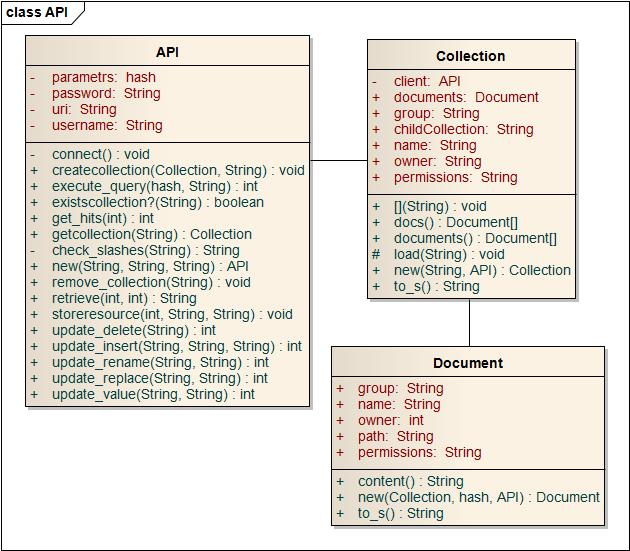
\includegraphics[width=15cm]{API1.jpg}
\caption{Diagram znázorňující model rozhraní}
\label{fig:API_interface}
\end{figure}

Na této části záleží bezpočenost. Potencionálně nebezpečné místo k útoku.

TODO Nekde je potreba nadefinovat co je Principal, Privilege a Resource Object

%----------------------------

\subsubsection{Rozhraní mezi Ruby-ACL a uživatelskou aplikací}
Rozhraní mezi knihovnou a uživatelskou aplikací tvoří všechny veřejné (public) metody třídy RubyACL. Pomocí instance této třídy a instance třídy API (která je předaná jako parametr) a následném volání veřejných metod může uživatel zavádět zmocnitele, oprávnění, zdrojové objekty a pravidla a pracovat s nimi.Výčet veřejných metod se nachází v příloze \ref{sec:veřejné metody}.

Nejčastěji používanou částí knihovny bude metoda \verb|check|. Mimo správu ACL objektů je hlavní účel knihovny rozlišit, jestli někdo nebo něco má oprávnění na nějaký zdrojový objekt. Pokud zmocnitel má nebo nemá přístup se uživatel dozví podle výstupu. Výstupem je true nebo false hodnota. Stručný popis nejčastějších vstupů a výstupů je v tabulce \ref{tab:tab3}

Rozhraní mezi Ruby-ACL a uživatelskou aplikací zproztředkovávají veřejné metody knihovny. To je patrné na obrázku diagramu komunikace \ref{fig:Communication diagram} v krocích 1 a 6.

\begin{table}%[h]
\centering
\begin{tabular}{|c|c|c|}
\hline
\textbf{jméno} & \textbf{typ} & \textbf{popis}\\
\hline
\multicolumn{3}{|l|}{Vstupy} \\
\hline
principal & string & jméno zmocnitele\\
\hline
privilege & string & název oprávnění\\
\hline
resource object type & string & typ - druh zdrojového objektu\\
\hline
resource object address & string & adresa zdrojového objektu\\
\hline
\hline
\multicolumn{3}{|l|}{Výstupy} \\
\hline
access & boolean & true = přístup povolen, false = přístup zakázán\\
\hline
\end{tabular}
\caption{Parametry a návratové hodnoty metody check} %\verb|check|}
\label{tab:tab3}
\end{table}

\subsection{Ukázka použití}
Tato sekce prezentuje stručné ale funkční ukázky použití. TODO vice textu?

\subsubsection{Příklad nastavení práv}
První příklad ukazuje, základní funkčnost knihovny a vytvoření pravidla. 
Protože knihovny Ruby-ACL vyžaduje jako jeden z parametrů instanci rozhraní API, bylo v příkladě použita implementace rozhraní eXistAPI. Pro vytvoření pravidla musí existovat instance Ruby-ACL. Ke správnému vytvoření pravidla je zapotřebí, aby všechny ACL objekty byly vytvořené. Pokud nebudou vytvořené, Ruby-ACL vyhodí vyjímku, nebo ACL Objekt založí. Metodě \verb|create_ace| je potřeba předat uživatelské jméno zmocnitele, typ přístupu (allow nebo deny), oprávnění a požadovaný objekt.


\begin{lstlisting}
require 'eXistAPI'    #must require 'eXistAPI' to comunicated with eXist-db
#creates instance of ExistAPI
@db = ExistAPI.new("http://localhost:8080/exist/xmlrpc", "admin", "password")    
@col_path = "/db/test_acl/"         #sets the collection where you want to have ACL in db
@src_files_path = "./src_files/"    #path to source files
@my_acl = RubyACL.new("my_acl", @db, @col_path, @src_files_path, true)
#it's good to create some principals at the begging
@my_acl.create_principal("Sheldon")
@my_acl.create_privilege("SIT")
@my_acl.create_resource_object("seat", "/livingroom/couch/Sheldon's_spot", "Sheldon")
@my_acl.create_ace("Sheldon", "allow", "SIT", "seat", "/livingroom/couch/Sheldon's_spot")
\end{lstlisting}


\subsubsection{Příklad kontroly práv}
Příklad tohoto kódu v podstatě říká: Pokud metoda \verb|acl_check| vratí hodnotu true, přístup povolen a aplikace provede co zamýšlela provést. Pokud vrátí hodnotu false, tak je přístup zamítnut. Tento postup názorně vysvětluje obrázek \ref{fig:Communication diagram} zobrazující komunikaci a průběh jednoho dotázení na pravidlo.


\begin{lstlisting}[firstnumber=12]
#Next method in if returns deny
if(@my_acl.check("Penny", "SIT", "seat", "/livingroom/couch/Sheldon's_spot"))
	puts "Access allowed. You may retrive resource object."
else
	puts "Access denied."
\end{lstlisting}

\subsection{Use Case Scénáře}
%\begin{verbatim}\end{verbatim}
\subsubsection{Ověřování oprávnění k objektu}
Uživatel má vytvořenou instanci RubyACL, která pracuje s pravidly.
Hlavní úspěšný scénář:
\begin{enumerate}
\item Uživatel zavolá metodu acl\_check. Přes tuto metodu se dotáže knihovny, jestli uživatel/skupina (ne)mají oprávnění ke zdrojovému objektu.
\item a) Systém vrátí true v případě, že uživatel/skupina má specifikované nebo vyšší oprávnění.
\item b) Systém vrátí false v případě, že uživatel/skupina nemají specifikované nebo vyšší oprávnění.
\end{enumerate}
Rozšíření:

0a) Pokud neexistuje žádné pravidlo, systém vrátí false, protože nenašel, žádné vyhovující pravidlo.
%\begin{verbatim}\end{verbatim}

\subsubsection{Zadávání pravidla (ACE)}
Uživatel má vytvořenou instanci RubyACL, která obsahuje pravidla.
Hlavní úspěšný scénář:
\begin{enumerate}
\item Uživatel zavolá metodu set\_new\_ace a specifikuje údaje (Uživatel/skupina, typ přístupy (allow/deny), oprávnění, zdrojový objekt
\item Knihovna nastaví pravidlo a vrátí 0, když vše proběhlo v pořádku, a 1 když nastala chyba.
\end{enumerate}
Poznámka: Jde vlastně o přiřazování oprávnění uživatelům na objekt



%-------------------------------------



\subsection{Data flow diagram}
TODO smazat starý obrázek. Okomentovat nový
Data flow diagram (viz "Obrázek 2") znázorňuje tok dat mezi jednotlivými funkcemi aplikace. Popisuje funkce a jejich vazby. Uložiště pro ACL je používaná databáze. Pro každou databázi bude jedna instance Ruby-ACL.
\begin{figure}
%\centering
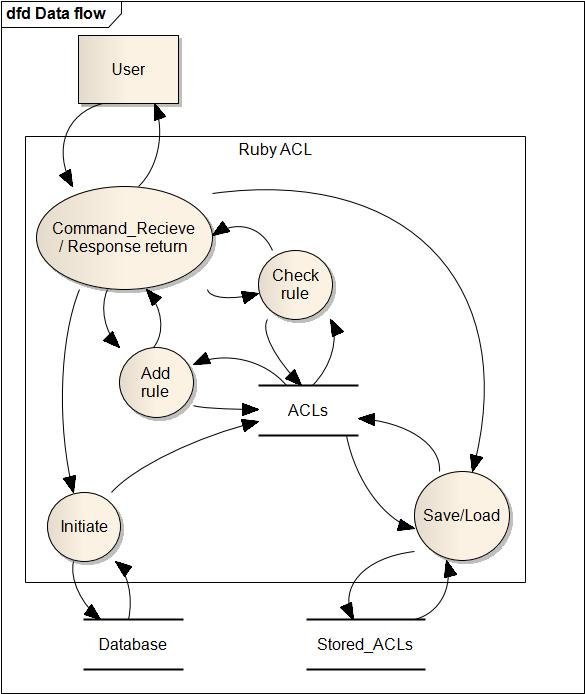
\includegraphics[width=15cm]{DataFlowBigFont.jpg}
\caption{Data flow diagram}
\label{fig:Data flow diagram}
\end{figure}

\begin{figure}
%\centering
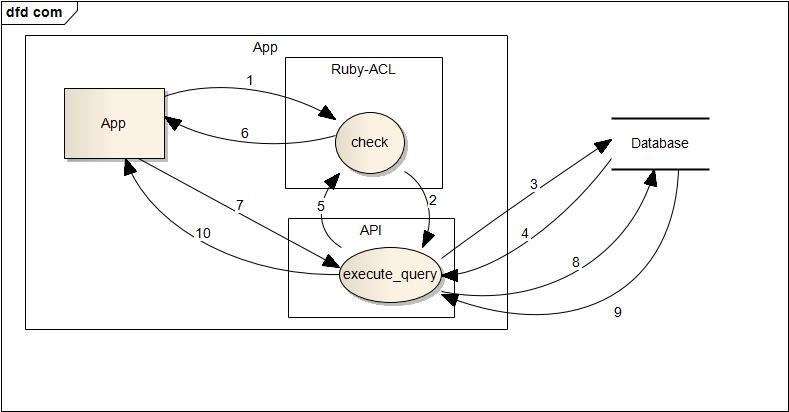
\includegraphics[width=15cm]{com.jpg}
\caption{Diagram znázorňující sekvenci komunikace}
\label{fig:Communication diagram}
\end{figure}

%-------------------------------------

\subsection{Class diagram}
Class diagram (viz "Obrázek 3") znázorňuje základní třídy aplikace a jejich vazby.
\begin{figure}
%\centering
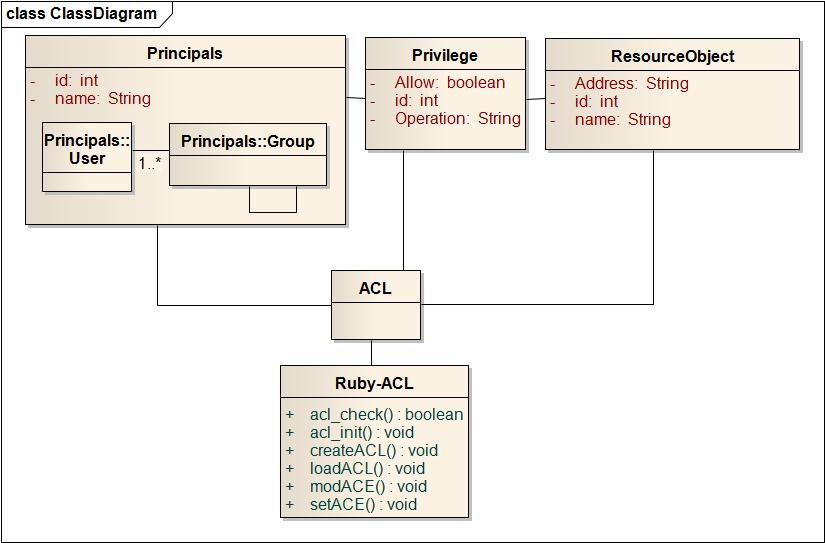
\includegraphics[width=15cm]{ClassDiagram2.jpg}
\caption{Class diagram}
\label{fig:Class diagram}
\end{figure}

%-------------------------------------
\section{Popis logiky vyhodnocování pravidel}
V této kapitole je popsáno jakým způsobem RubyACL rozhoduje o přidělení přístupu. Nejkonkrétněji se tímto zabývá sekce "Pravidla rozhodování", nicméně k pochopení celku je potřeba vědět vlastnosti jednotlivých objektů, které jsem nazval ACL objekty. O nich se dočtete ve stejnojmenné sekci.
Vše se odvijí od priority rozhodování.

\subsection{ACL Objekty}
ACL objekt je principal, který se dělí na individual a group, privilege

\subsubsection {Zmocnitel (Principal)}
Principal = [Individual, Group]
\begin{verbatim}
        <Group id="Administrators">
            <membership>
                <mgroup idref="ALL"/>
            </membership>
        </Group>
        <Individual id="sirljan">
            <membership>
                <mgroup idref="Users" />
                <mgroup idref="Developers" />
            </membership>
        </Individual>
\end{verbatim}

\subsubsection {Oprávnění (Privilege)}
RubyACL obsahuje základní oprávnění Oracle a MySQL. Nevím ale, jestli to bude mít nějaký význam, když XML databáze má jinou formu dotazování. 
Pravidla lze jednoduše vytvořit a seskupovat.
Ruby-ACL nabídne vlastní přidané privilegia a základní sadu privilegií a převzatých z Oracle potažmo MySQL. Jedná se o privilegia 'ALL PRIVILEGES', 'ALTER', 'CREATE', 'DELETE', 'DROP', 'FILE', 'INDEX', 'INSERT', 'PROCESS', 'REFERENCES', 'RELOAD', 'SELECT', 'SHUTDOWN', 'UPDATE' a 'USAGE'.
\begin{verbatim}
    <Privilege id="SELECT">
        <membership>             
            <mgroup idref="ALL_PRIVILEGES" />         
        </membership>
    </Privilege
\end{verbatim}

\subsubsection {Zdrojový objekt (Resource object)}
Skládá se ze tří položek:
\begin{enumerate}
\item typ
\item adresa
\item vlastník
\end{enumerate}

Při zadávání adresy je potřeba dodržet jediné pravidlo. V adrese oddělovat každý jednotlivý objekt dopředným lomítkem. ( / )

Pokud je zdrojový objekt typu doc, adresa může obsahovat klauzuli ve formátu ("/koren/vetev/list-soubor\_s\_příponou") a pokud je zapotřebí jemnější řízení přístupu uvnitř dokumentu následuje klauzule /koren/vetev. Nicméně do databáze se ukládá sloučená adresa bez ("")
Příklad:  ("/db/data/cities.xml")/cities/city
V databázi je uložen pod adresou: /db/data/cities.xml/cities/city

Klauzule /* (lomítko hvězdička) vyjadřuje všechny podřadné objekty
Příklad:  /db/data/*
Nyní jsou vybrány všechny podřadné objekty objektu data.
/* nemá význam u vlastníka, protože vlastník zdrojového objektu vlastní i všechny podřazené zdrojové objekty.

Vlastník / Owner
Owner může být jednotlivec, množina jednotlivců i skupina.
Množina jednotlivců je v případě pokud se od kořene zdrojových objektů k listu mnění vlastník. Vlastník nejnadřazenějšího zdroje má největší práva. Vlastník může být o 
/* nemá význam, protože vlastník zdrojového objektu vlastní i všechny podřazené zdrojové objekty.

\subsubsection{Pravidlo (ACE)}
\begin{verbatim}
        <Ace id="a894">
            <Principal idref="Users"/>
            <accessType>allow</accessType>
            <Privilege idref="SELECT"/>
            <ResourceObject idref="852"/>
        </Ace>
\end{verbatim}

\subsection{Složitost rozhodování}
Slozitost je e\^2.

%--------------------------------

\subsection{Pravidla rozhodování}
\subsubsection{Priorita rozhodování}

Nejnižší má největší prioritu.

\begin{enumerate}
\item Owner
\item Explicit Deny
\item Explicit Allow
\item Inherited Deny
\item Inherited Allow
\item If not found > Deny
\end{enumerate}


%*****************************************************************************
% Realizace
\chapter{Realizace}
Popis implementace/realizace se zaměřením na nestandardní části řešení.

\section{Průběh realizace}
Průběh realizace jsem si zpětně rozdělil do několika fází, tak jak šly chronologicky po sobě. Každá fáze představuje určitou etapu ve vývoji knihovny.
\\
\\
\noindent Fáze 1

\noindent Po analýze a návrhu byla naimplementována zkušební část kvůli ověření návrhu tříd a rozhraní. Na tuto verzi byla napsána první velká skupina unit testů. Verze nepracovala vůbec s databází, byla pouze instanční a od současného modelu tříd se velmi odlišovala. Tato část práce byla součástí mého softwarového projektu.
\\
\\
\noindent Fáze 2

\noindent Po dokončení instanční verze jsem pokračoval seznámením se s databází eXist-db, která mi byla doporučena vedoucím práce. V této fázi nastaly největší potíže. Nemohl jsem najít způsob, jak komunikovat s databází. V Ruby neexistovalo žádné komunikační rozraní, které by umožňovalo měnit obsah a dotazovat se na něj. Dokumentace přímo na webu \cite{exist:exist} popisovala jenom protokoly, kterými lze s databází komunikovat. Mezi ně patří napríklad REST\footnote{Representational State Transfer}, SOAP\footnote{Simple Object Access Protocol} a XML-RPC, který jsem si zvolil pro vývoj API. Velice mi pomohlo, nalezení ukázky knihovny pro XML-RPC v instalačním adresáři eXist-db. 

Komplikace tím neskončily. Uměl jsem sice pomocí XML-RPC pracovat s kolekcemi a dokumenty, ale nedokázal jsem pomocí XUpdate upravovat dokumenty: vkládat, upravovat a mazat uzly a atributy. Dodržel jsem dokumentaci XML-RPC, specifikace metody \verb|XUpdate| \cite{exist:xmlrpcxupdate} a dokumentaci XUpdate \cite{xupdate}, na kterou se eXist odvolává. V této fázi se mi delší dobu nedařilo zprovoznit upravování dokumentů. Proto jsem začal vyhledávat alternativní možnosti. Hledal jsem XML databázi, která by měla komunikační rozhraní v Ruby. Našel jsem jedinou databázi jménem Sedna. Bohužel ani s ní jsem nedospěl pokroku. Problém byl se zprovozněním knihoven, které byly napsané v jazyku C.

Významnou pomocí v této fázi pro mě byla rada vedoucího mojí bakalářské práce Ing. Strnada, který mě nasměroval na použití technologie XQuery Update Facility.
\\
\\
\noindent Fáze 3

\noindent Přepracoval jsem první verzi implementace RubyACL z lokální/instanční na databázovou, což představovalo přepsání tříd na pseudo-singletonské managery. Třídy nejsou čistými singletony, ale knihovna obsahuje pouze jednu instanci od každé pomocné třídy. Všechny informace jsou uloženy v databázi. RubyACL pouze vkládá nové záznamy, upravuje a maže staré. Na existujících záznamech provádí dotazy a rozhodování o přístupu. Při úplném naimplementování eXistAPI, jsem kompletně předělal třídní model. Do této doby byly třídy jako Principal, Privilege, ResourceObject a ACE používány pro ukládání dat do instancí a polí instancí. Ve fázi 3 jsem tyto třídy předělal na pomocné třídy, které upravují pomocí poskytnutého rozhraní obsah databáze. Přidal jsem třídy Individual a Group. Dalším nezdarem v této části bylo vytvoření nějakého referenčního systému mezi ACL objekty.  Pro identifikaci a propojení jsem uvažoval mezi xLink a idref. Idref nabízí jednoduchý systém, ale xLink nabídl podrobné specifikace W3C, velké množství návodů a turtoriálů a především se jedná o novější technologii, jejíž osvojení jsem považoval za výhodné. Rozhodl jsem se proto implementovat xLink. Problém nastal při některých vkládání textů a dotazování. eXist-db měla problém s jmenným prostorem xLink i přes skutečnost, že jmenný prostor byl uveden jak v samotném XML dokumentu, tak ve vkládaném uzlu. I když jsem se zabýval, proč použití xLink nejde, nedospěl jsem rozřešení a tak jsem raději přešel na jednoduchý idref. Implementace idref proběhla rychle a bez problémů.
\\
\\
\noindent Fáze 4

\noindent Druhý návrh tříd nebyl zcela správný a i implementace se odchylovala od návrhu. Znovu jsem musel zasáhnout do modelu tříd a předělat jej. Vytvořil jsem nadřazenou třídu \verb|ACL_Object|, ze které dědí ostatní pomocné třídy. V této fázi jsem velmi intenzivně testoval. Opakované ověřování správné funkčnosti při neustálém upravování knihovny, mi zabíralo příliš mnoho času. V této fázi jsem docenil význam unit testů a jejich schopnost odhalovat chyby.
\\
\\
\noindent Fáze 5

\noindent Dokončil jsem rozhodovací metodu \verb|check| a dotáhl do finální podoby funkcionality knihovny. V této fázi jsem opravil chyby a odstranil nedostatky. Přidal jsem další velkou část unit testů, převážně zaměřených na metodu \verb|check|. Začal jsem tvořit dokumentaci.
\\
\\
\noindent Fáze 6

\noindent Vydal jsem Ruby-ACL a eXistAPI jako RubyGem a odzkoušel na nezávislém počítači. Dokončil jsem dokumentaci. 


\section{Programy použité při vývoji}
V následujícím seznamu jsou uvedeny všechny programy, které jsem při vývoji knihovny použil.
\begin{itemize}
\item NetBeans s Ruby platformou od Thomase Enebo
\\
\url{http://blog.enebo.com/}
\\
\url{http://plugins.netbeans.org/plugin/38549/ruby-and-rails}
\item GIT
\url{https://github.com/sirljan/Ruby-ACL}
\item eXist-db
\url{http://www.exist-db.org}
\item Enterprise Architect
\item MikTex
\end{itemize}
%-------------------------------------
\section{Databáze}
Protože XML databáze, která má RubyACL používat, není dosud plně funkční, nebylo možné implementaci testovat přímo na ní. Za tímto učelem se musela vybrat jiná podobná databáze.

\subsection{Sedna}
Databáze Sedna poskytuje rozhraní v Ruby. Klientské rozhraní je Ruby rozšíření, které používá ovladač jazyka C, který je dodáván jako součást distribuce Sedna. Použití má být jednoduché a snadno použitelné. Ovšem zprovoznění knihovny Sedna je nedostatečně popsané a nekompatibilní se současnou verzí Ruby 1.9.3.

\subsection{eXist-db}
Open source systém eXist-db je systém pro správu databáze vytvořené pomocí technologie XML. Databáze eXist-db ukládá XML data podle datového modelu XML a nabízí efektivní a XQuery zpracování založené na indexování. Podporuje velké množství technologií. Dále zde uvádím pouze ty, které se týkají RubyACL nebo eXistAPI: XPath 2.0, XQuery, XML-RPC, XQuery Update Facility 1.0. 

eXist-db se podobá XML databázi, která má RubyACL používat, a byla doporučena vedoucím práce jako ideální. Přesto se vyskytly komplikace s XUpdate navzdory přesné interpretace dokumentace. Z tohoto důvodu bylo nutné přejít na XQuery Update Facility.

\subsubsection{eXistAPI}
ExistAPI je komunikační rozhraní, jehož implementaci si vynutilo ladění a testování knihovny RubyACL na databázi eXist-db. Jednalo se o trochu nestandartní část realizace, protože eXist-db nemá knihovnu rozhraní pro jazyk Ruby.

eXistAPI komunikuje s databází prostřednictvím XML-RPC protokolu a technologíí XQuery a XPath. XQuery Update Facility se používá pro editování dat v dokumentech kolekcí databáze.
Pokus o naimplementování XUpdate nebyl úspěšný. XUpdate není podporován konzorciem W3C\footnote{World Wide Web Consortium} a tudíž není jednoznačně nadefinovaný. Zde nejspíše vznikl problém, kdy eXist-db použila jinou interpretaci XUpdate, než uvádí dokumentace XUpdate \cite{xupdate}.

Interface eXistAPI považuji za přínos pro uživatele eXist-db, kteří programují v Ruby. Rozhraní eXistAPI je ošetřené výjimkami, otestované a zdokumentované tak, jak to vyžaduje balíčkovací systém \href{https://rubygems.org/}{RubyGem}, kde ho lze najít pod jménem "eXistAPI". Lze jej tedy stáhnout příkazem \verb|gem install eXistAPI|. Model tříd je v příloze \ref{fig:eXistAPI}. 

%-------------------------------------
\section{Implementace}
V této sekci se zabývám popisem implementace metody \verb|check| a popsáný příklad založení uživatele.

\subsection{Třída RubyACL}

Hlavní účel třídy \verb|RubyACL| je zprostředkovávat funkčnost pomocných tříd dědících z třídy \verb|ACL_Object|. Dále třída \verb|RubyACL| nabízí možnost ukládání a načítání ACL ze souborů a hlavně obsahuje metodu \verb|check|, která slouží k vyhodnocování pravidel.

\subsubsection{Metoda check}
Metoda check obstarává rozhodování, jestli zmocnitel má oprávnění k objektu nebo nemá. Stručně a výstižně vysvětluje algoritmus obrázek \ref{fig:check}. 

Metoda \verb|check| nejprve zjistí, jestli daný zmocnitel není vlastník daného objektu nebo jakéhokoliv nadřazeného objektu. Pokud je vlastníkem, ihned vratí true a ukončí běh. 
Pokud zmocnitel není vlastníkem, metoda \verb|check| nashromáždí všechna potenciální pravidla, která by mohla ovlivňovat přístup. Udělá to tak, že pro daného zmocnitele najde všechny jeho nadřezené zmocnitele. Jedná se tedy o pole skupin a pokud je daným zmocnitelem jednolivec, tak i on. Obdobným způsobem vytvoří i pole privilegií a nadřazených privilegií, zdojových objektů a nadřazených zdrojových objektů. Dále z těchto polí vytvoří XQuery dotaz, který vybere takové pravidlo, které obsahuje jednoho ze zmocnitelů a zárověn jedno z pravidel a zároveň jeden zdrojový objekt. XQuery se odešle pomocí eXistAPI a přijme se množina pravidel. V této množině pravidel hledá metoda \verb|check| pravidlo, které má nejvyšší prioritu. Metoda určuje prioritu podle seznamu v sekci \ref{Priorita rozhodování} Priorita rozhodování. Metoda prochází pravidla a srovnává pravidlo uložené v pomocné proměnné s aktuálním pravidlem. Pokud aktuální pravidlo má větší prioritu je zapsáno do pomocné proměnné. Pokud není žádný další záznam, metoda přečte \verb|accessType| a podle něj rozhodne, co vrátí. Pokud \verb|accessType| obsahuje "allow" vrátí true, pokud obsahuje "deny" vrátí false.
\begin{figure}
%\centering
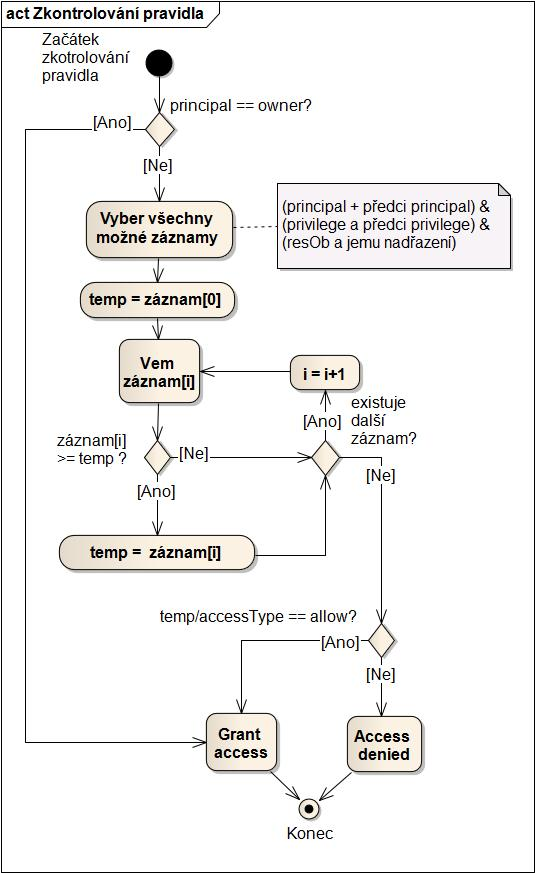
\includegraphics[width=15cm]{check2.jpg}
\caption{Diagram znázorňující chod metody check}
\label{fig:check}
\end{figure}

\subsubsection{Příklad}
\label{Příklad}
Uvedu zde jeden příklad vytvoření zmocnitele a na něm popisuji průchod logikou knihovny.
\\
\lstset{language=Ruby, numbers=none}
\begin{lstlisting}
@my_acl.create_principal("Sheldon", "4th_Level")
\end{lstlisting}

Je zřejmé, že příkaz volá metodu \verb|create_principal|. Příkaz má vytvořit zmocnitele jménem \verb|"Sheldon"|, který bude patřit do skupiny \verb|"4th_Level"|. \verb|RubyACL| má instanci od každé pomocné třídy. \verb|RubyACL| tedy pouze zavolá metodu \verb|create_new| instance \verb|@indi|, což je instance třídy \verb|Individual|. Metoda \verb|create_new| ničím nekonkretizuje chování supertřídy \verb|ACL_Object|, takže se zavolá metoda této třídy. Zde se provede kotrola, jestli jméno není prázdné. Pokud jméno je prázdné, vyhodí se výjimka. Dále se pokračuje kontrolou, jestli jméno už není obsazené. Pokud je, vyhodí se výjimka. Pomocí metody \verb|generate_expr| se vygeneruje uzel, který bude následně vkládat. Metoda \verb|generate_expr| není ve třídě \verb|Individual| přepsaná (anglicky overridden), takže se v tomto případě volá metoda supertřídy. Výsek kódu tvoření uzlu je v následující ukázce:
\\
\begin{lstlisting}
    expr = <<END
    <#{self.class.name} id="#{name}">
      <membership>
        
      </membership>
    </#{self.class.name}>
END
\end{lstlisting}
Kód ukazuje, že jméno uzlu je utvořeno podle jména třídy (jedná se o část \verb|self.class.name|), takže jméno uzlu je v tomto případě "Individual". Dalším krokem je vytvoření části příkazu, který rozhoduje, kam se uzel bude vkládat a opět se využívá jména třídy.
\\
\begin{lstlisting}
expr_loc = "#{@doc}//#{self.class.name}s/#{self.class.name}[last()]"
\end{lstlisting}
Zbývá už pouze zavolat metodu \verb|update_insert| instance třídy \verb|eXistAPI|, která vloží připravený uzel na připravenou pozici. Následně se zkontroluje, pokud byl uzel vložen, pokud ne, vyvolá se výjimka.

Následuje větvení, které rozhoduje zda se bude zmocnitel přidávat do nějaké skupiny. V tomto případě se zmocnitel do skupiny bude přidávat. Přidávání se provádí pomocí metody \verb|add_membership|, kterou lze volat i samostnatně. Parametry metody jsou: "kdo má být", "v jaké skupině". Metoda zjednodušeně řečeno vkládá do zmocnitele odkaz na skupinu. Metoda \verb|add_membership| funguje podobně jako \verb|create_new|. Připraví se uzel na vkládání, lokace vložení jako XPath výraz a předtím než se zavolá \verb|update_insert| se zkontroluje, jestli se členství necyklí. Nakonec se zkontroluje, jestli byl uzel vložen, pokud ne, vyvolá se výjimka.


%-------------------------------------

\subsection{ACL\_Object}
Třída \verb|ACL_Object| je rodičem tříd: Principal, Privilege, ResrouceObject, ACE a nepřímým rodičem Individual a Group.
Třída sdružuje obecné metody, které jsou společné pro všechny výše vyjmenované třídy. Takové metody například jsou: \verb|create_new|, \verb|delete|, \verb|rename|. \\ \verb|ACL_Object| také obsahuje důležitou proměnou \verb|doc|, která obsahuje cestu k datovému dokumentu v databázi. Tuto proměnnou taktéž třídy dědí.
Jednotlivé třídy vyjmenované v této sekci pracují se svým dokumentem. Dokument a uzly v něm mají různou strukturu. Například oprávnění má jeden kořenový uzel a pak už jen seznam oprávnění, ve kterých jsou odkazy na nadřazená oprávnění. Jedná se o poměrně jednoduchou strukturu ve srovnání s ostatními datovými dokumenty. Každá ze tříd má tuto strukturu v sobě uloženou a podle ní tvoří dotazy na editování dat.

%-------------------------------------

\subsection{Výjimky}
Výjimky pro knihovnu RubyACL vyvolává třída \verb|RubyACLException|. Knihovna buď výjimky vyvolává nebo je jen propaguje dále. Seznam výjimek, jejich kódů a metod, které je vyvolávají jsou vypsané na přiloženém CD přímo pod zdrojovým kódem třídy \verb|RubyACLException| a \verb|ExistException|.

\noindent Výjimky pro rozhraní eXistAPI vyvolává třída \verb|ExistException|.

%-------------------------------------

\subsection{Práce s pamětí}
Už od začátku mojí práce bylo jasné, že bych neměl zanedbat správu paměti, protože aplikace s knihovnou bude spuštěna v řádech dnů a měsíců. Špatné zacházení s pamětí by proto bylo kritické pro server, na kterém aplikace s Ruby-ACL knihovnou bude spuštěna. Ruby-ACL veškera data ukládá do databáze. Jediné obsazení paměti je instancí samotné třídy \verb|RubyACL| a instancemi pomocných tříd. Nicméně v Ruby uvolňování paměti programátorem nemá význam, protože v dynamickém prostředí Ruby se o uvolňování stará garbage collector. Ruby používá garbage collector, který nepoužívané objekty vystopuje a odstraní \cite{Ruby}.

%*****************************************************************************
% Testování
\chapter{Testování}

\begin{itemize}
 \item Způsob, průběh a výsledky testování.
 \item Srovnání s existujícími řešeními, pokud jsou známy.
\end{itemize} 


Testování bylo zaměřeno pouza na funkcionalitu. Vynecháno bylo testování rychlosti, práce s operační pamětí, spotřeby procesorového času. 


\section{eXistAPI}
\section{RubyACL}

%*****************************************************************************
% Závěr
\chapter{Závěr}

\begin{itemize}
\item Zhodnocení splnění cílů DP/BP a  vlastního přínosu práce (při formulaci je třeba vzít v potaz zadání práce).
\item Diskuse dalšího možného pokračování práce.
\end{itemize} 

Možné zlepšení: 
rychlost - Jednoznačně časově nejdražší operací je komunikace s databází. Zrychlení by se dalo docílit optimalizací dotazování tak, aby se dotazovalo, co nejméně. Daňí by byla větší paměťová náročnost aplikace, která by knihovnu RubyACL používala. Současný kód knihovny obsahuje opakované dotazování na stejnou věc místo ukládání výsledku do paměti pro případné následující použití. Tento model byl zvolen kvůli jednoduchosti a faktu, že vykonání dotazu a vrácení výsledku trvá řadově milisekundy. Je ale těžké odhadnout, kolik času by zabralo dotazování při plné databázi a použití více uživatelů ve stejný čas. Navíc eXist si po určitou dobu v paměti uchovává výsledky předchozích dotazů, čímž se snižuje naročnost opakovaných dotazů. Vše je ale závislé na lince mezi knihovnou a databází.

%*****************************************************************************
%\chapter{Literatura}
% Seznam literatury je v samostatnem souboru reference.bib. Ten
% upravte dle vlastnich potreb, potom zpracujte (a do textu
% zapracujte) pomoci prikazu bibtex a nasledne pdflatex (nebo
% latex). Druhy z nich alespon 2x, aby se poresily odkazy.

% originally following specification for bibliography formating was used
%\bibliographystyle{abbrv}

% Here is an improvment by Petr Dlouhy (April 2010).
% It is mainly for supervisors who expect Czech fomrating rules for references
% Additional feature is live url addresses to sources from your pdf file
% It requires the file csplainnat.bst (included in this sample zipfile).

\bibliographystyle{csplainnat}

%bibliographystyle{plain}
%\bibliographystyle{psc}
{
%JZ: 11.12.2008 Kdo chce mit v techto ukazkovych odkazech take odkaz na CSTeX:
\def\CS{$\cal C\kern-0.1667em\lower.5ex\hbox{$\cal S$}\kern-0.075em $}
\bibliography{reference}
}

% M. Dušek radi:
%\bibliographystyle{alpha}
% kdy citace ma tvar [AutorRok] (napriklad [Cook97]). Sice to asi neni  podle ceske normy (BTW BibTeX stejne neodpovida ceske norme), ale je to nejprehlednejsi.
% 3.5.2009 JZ polemizuje: BibTeX neobvinujte, napiste a poskytnete nam styl (.bst) splnujici citacni normu CSN/ISO.

%*****************************************************************************
%*****************************************************************************
\appendix

%*****************************************************************************
\chapter{Výpis veřejných metod Ruby-ACL}
\label{sec:veřejné metody}
V této sekci se nachází výpis veřejných metod. Všechny metody i s parametry a návratovými hodnotami je možné najít v RDOC dokumentaci na CD.
\begin{itemize}
\item \verb|new|
\item \verb|add_membership_principal|
\item \verb|add_membership_privilege|
\item \verb|change_of_res_ob_address|
\item \verb|change_of_res_ob_owner|
\item \verb|change_res_ob_type|
\item \verb|check|
\item \verb|create_ace|
\item \verb|create_group|
\item \verb|create_principal|
\item \verb|create_privilege|
\item \verb|create_resource_object|
\item \verb|del_membership_principal|
\item \verb|del_membership_privilege|
\item \verb|delete_ace|
\item \verb|delete_principal|
\item \verb|delete_privilege|
\item \verb|delete_res_object|
\item \verb|delete_res_object_by_id|
\item \verb|rename|
\item \verb|rename_principal|
\item \verb|rename_privilege|
\item \verb|save|
\item \verb|show_permissions_fo|
\end{itemize}

%*****************************************************************************
\chapter{Seznam použitých zkratek}

\begin{description}
\item[ACL] Access Control List
\item[ACE] Access Control Entry
\item[XML] Extensible Markup Language
\item[RDOC] RubyDOCumentation
\item[ACO] Access Control Objects
\item[ARO] Access Request Objects
\item[API] Application Programming Interface
\item[phpGACL] Generic Access Control Lists with PHP
\item[DTD] DTD
\item[XML-RPC] XML Remote Procedure Call protokol
\item[xQuery] Dotazovací jazyk nad XML dokumenty
\item[XPath] XML Path Language
\item[W3C] World Wide Web Consortium
\item[irb] Interactive Ruby Shell
\item[JDK] Java Development Kit
\end{description}

%*****************************************************************************
\chapter{UML diagramy}

Vytvořené diagramy jsem tvořil podle knihy Destilováné UML \cite{UML}

\section{Use Case Diagram}
Znázorňuje roli uživatele vůči knihovně. Ruby ACL definuje jednoho aktéra, kterým je uživatel/administrátor ACL viz obrázek \ref{fig:usecase}. Jedná se vlastně o vývojáře DB Applikace.
Všechny případy užití předpokládají vytvořenou instanci RubyACL, která má vytvořená nějaká pravidla.
\begin{figure}
%\centering
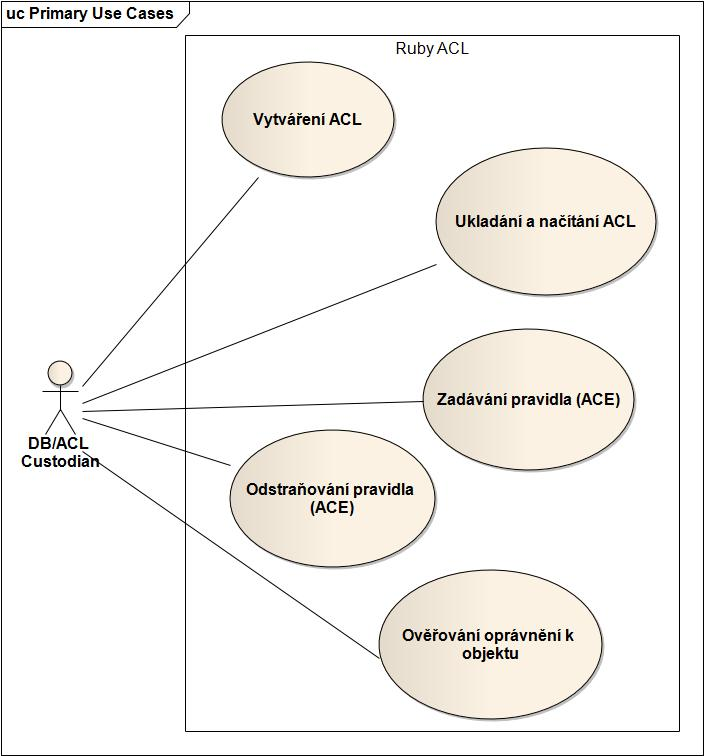
\includegraphics[width=15cm]{UseCases.jpg}
\caption{UseCases}
\label{fig:usecase}
\end{figure}

\section{eXistAPI}
Obrázek popisuje třídní model rozraní eXistAPI.
\begin{figure}
%\centering
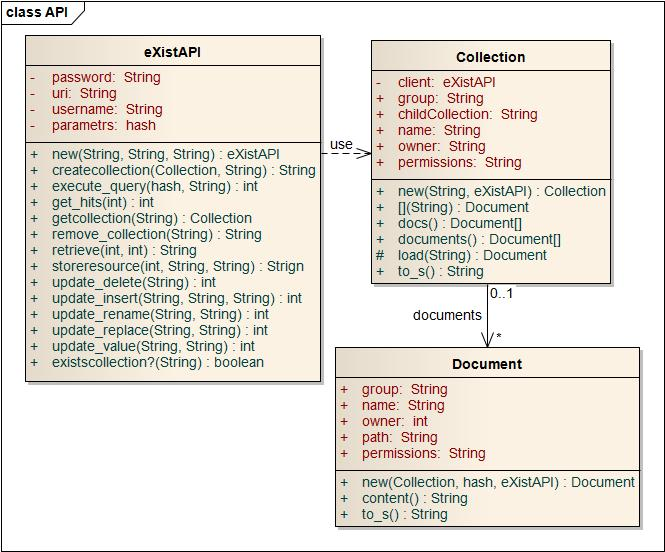
\includegraphics[width=15cm]{eXistAPI.jpg}
\caption{Diagram tříd eXistAPI}
\label{fig:eXistAPI}
\end{figure}

%-------------------------------------

%*****************************************************************************
\chapter{Instalační a uživatelská příručka}

Pro úspěšné zprovoznění mnou naimplementované knihovny, která spravuje přístupová práva, musíte nejprve nainstalovat software, na kterém je knihovna závislá. Jedná se o:
\begin{itemize}
\item Ruby prostředí - \url{http://www.ruby-lang.org/en/downloads/}
\\ Na příslušné stránce vyberte distribuci podle vašeho operačního systému. Pro windows je nejlepší řešení RubyInstaller. Nainstalujte nejnovější verzi. V době vydání knihovny byla nejnovějčí verze Ruby 1.9.3.-p194.  Při instalaci zaškrtněte "Add Ruby executables to your PATH"
\item JDK \href{http://www.oracle.com/technetwork/java/javase/downloads/jdk-7u4-downloads-1591156.html}{JDK}
\\ Databáze eXist-db pro svůj běh potřebuje Java Development Kit. JRE není dostačující.
\item Databázi eXist-db - \url{http://exist-db.org/exist/download.xml}
\\ Doporučuji stáhnout "Stable release". V době vydání byla dostupná verze eXist-setup-1.4.2-rev16251.
\end{itemize}

Dále potřebujete nainstalovat samotnou knihovnu a eXistAPI rozhraní.
Nejjednodušším způsobem, jak nainstalovat knihovnu a komunikační rozhraní pro eXist-db, je nainstalovat Ruby prostředí včetně balíčkovacího systému gem a nainstalovat jak knihovnu, tak rozhraní pomocí příkazů \verb|gem install Ruby-ACL| (pomlčka je podstatná, protože "rubyacl" je gem, který s mojí knihovnou nemá nic společného) a \verb|gem install eXistAPI|. Příkazy lze použít ve standartní příkazové řádce, pokud jste zaškrtli při instalaci volbu "Add Ruby executables to your PATH". 

Dalším způsobem, jak používat knihovnu s rozhraním je, stáhnout si zdrojové kódy buď z CD nebo z githubu. Zdrojové kódy Ruby-ACL se nachází na \url{https://github.com/sirljan/Ruby-ACL} a zdrojové kódy eXistAPI jsou na \url{https://github.com/sirljan/eXistAPI}. V případě stažení kódu z githubu je důležité použít příkaz \verb|require| se správnou adresou ke zdrojovým souborům. 

\noindent Poznámka: Výchozí adresy, ze kterých \verb|require| vkládá soubory, jsou aktuální adresář a adresář, kde se ukládají gem. Proto, když si gem nainstalujete přes rubygem, není potřeba řešit adresy, stačí použít příkazy \verb|require 'Ruby-AL'| a \verb|require 'eXistAPI'|.

\noindent Před použitím spusťte eXist-db. Funkčnost můžete ověřit třeba v \verb|irb|\footnote{Interactive Ruby Shell} zavoláním příkazů:

\begin{verbatim}
require 'Ruby-ACL'
require 'eXistAPI'
@db = ExistAPI.new("http://localhost:8080/exist/xmlrpc", "admin", "password")
@my_acl = RubyACL.new("my_acl", @db)
@my_acl.create_principal("Sheldon")
\end{verbatim}

Po spuštění těchto příkazů najdete pomocí eXist Admin Clientu, v kolekci \verb|"/db/acl/"| dokument  \verb|Principals.xml|, ve kterém by měl být (jako poslední v uzlu Individuals) uzel s id="Sheldon". Pokud uzel v dokumentu není, něco bylo chybně provedeno.

%*****************************************************************************
\chapter{Obsah přiloženého CD}
\textbf{\large Tato příloha je povinná pro každou práci. Každá práce musí totiž obsahovat přiložené CD. Viz dále.}

Může vypadat například takto. Váš seznam samozřejmě bude odpovídat typu vaší práce. (viz \cite{infodp}):

\begin{figure}[h]
\begin{center}
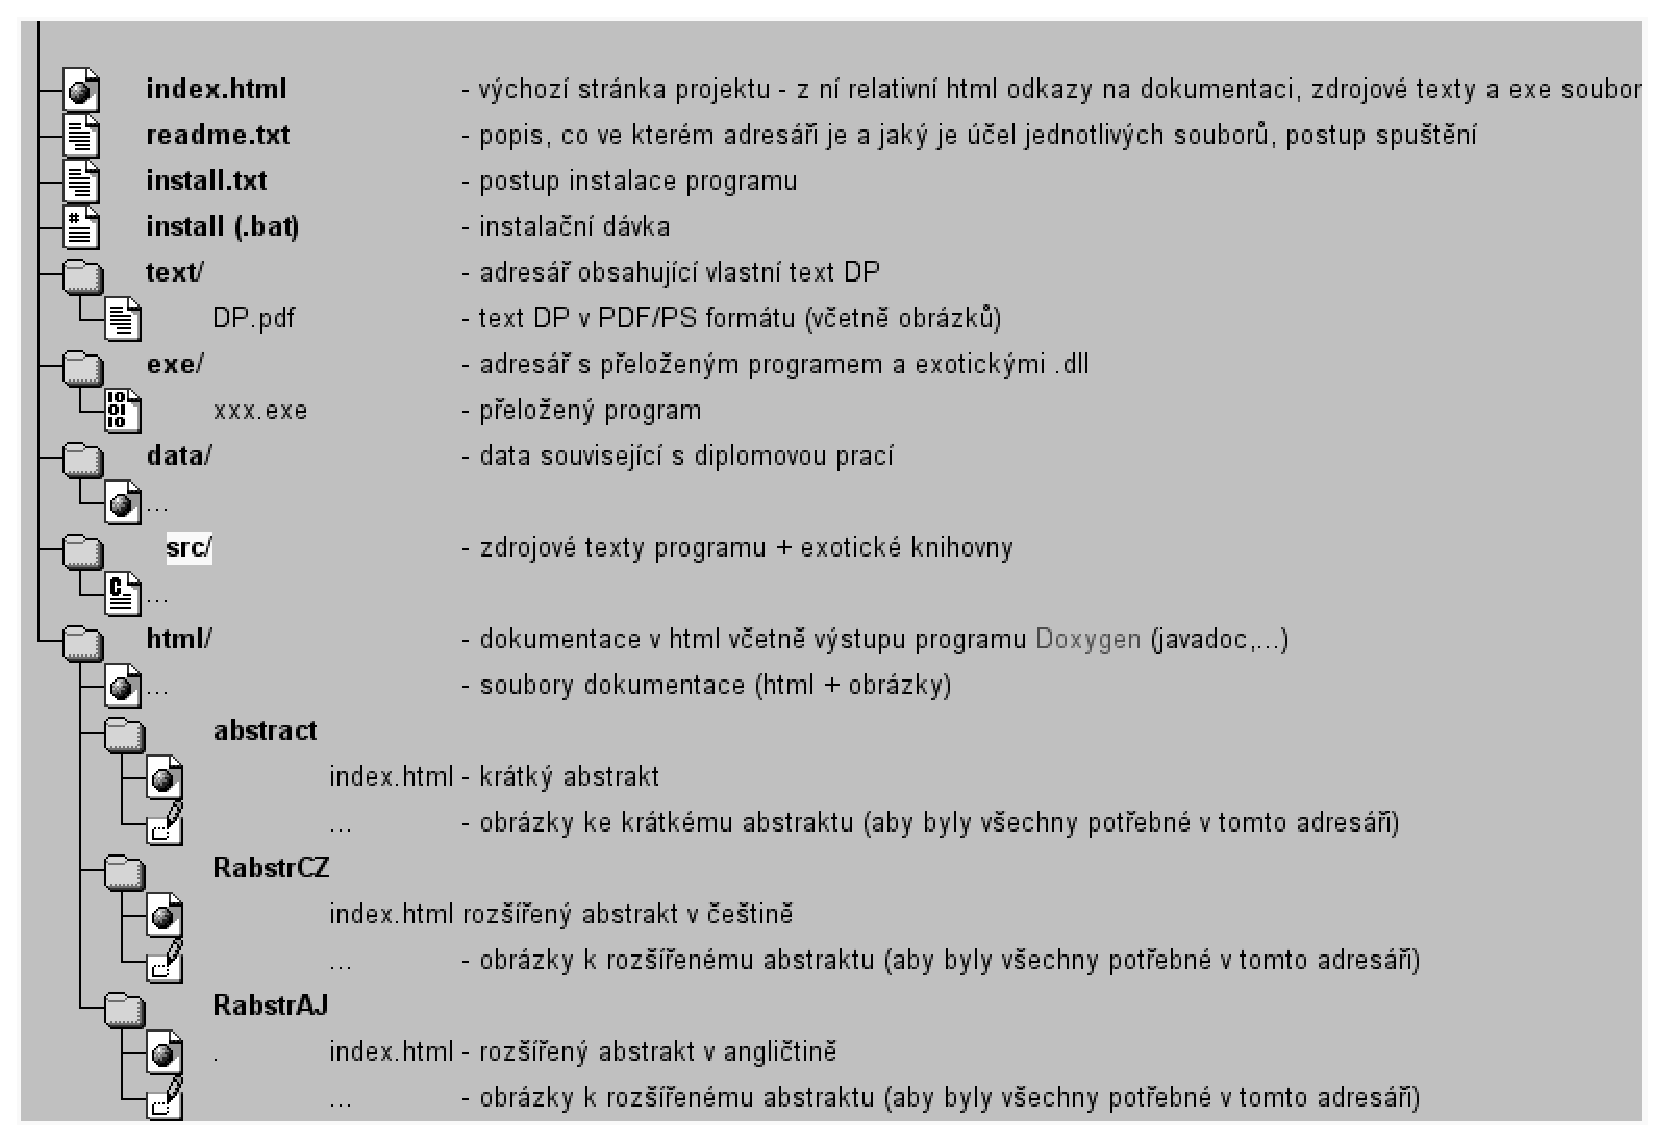
\includegraphics[width=14cm]{figures/seznamcd}
\caption{Seznam přiloženého CD --- příklad}
\label{fig:seznamcd}
\end{center}
\end{figure}

Na GNU/Linuxu si strukturu přiloženého CD můžete snadno vyrobit příkazem:\\ 
\verb|$ tree . >tree.txt|\\
Ve vzniklém souboru pak stačí pouze doplnit komentáře.

Z \textbf{README.TXT} (případne index.html apod.)  musí být rovněž zřejmé, jak programy instalovat, spouštět a jaké požadavky mají tyto programy na hardware.

Adresář \textbf{text}  musí obsahovat soubor s vlastním textem práce v PDF nebo PS formátu, který bude později použit pro prezentaci diplomové práce na WWW.

\begin{verbatim}
.
|-- abstract                     - adresář s abstraktem v čj a aj
|   |-- abstract.html            - krátky abstract
|   |-- RabstractAJ.html         - rozšířený abstract v angličtině
|   `-- RabstractCZ.html         - rozšířený abstract v češtině
|-- gem                          - adresář obsahující instalační balíčky gem
|-- index.html                   - výchozí stránka projektu - z ní realtivní 
|                                   html odkazy na dokumentaci, zdrojové 
|                                   texty a exe soubor
|-- install.TXT                  - postup instalace knihovny
|-- rdoc                         - adresář s rdoc dokumentací
|   |-- eXistAPI                 - rdoc dokumentace k eXistAPI
|   |   |-- index.html           - výchozí stránka dokumentace eXistAPI  
|   |   `-- ...                  - další soubory a stránky dokumentace
|   |   |-- images               - obrázky/ikony dokumentace
|   |   |   `-- ...
|   `-- Ruby-ACL                 - rdoc dokumentace k Ruby-ACL
|       |-- index.html           - výchozí stránka dokumentace Ruby-ACL 
|       `-- ...                  - další soubory a stránky dokumentace
|       |-- images               - obrázky/ikony dokumentace
|           `-- ...
|-- readme.TXT                   - popis, co ve kterém adresáři je a jaký je účel 
|                                   jednotlivých souborů, postup spuštění
|-- src                          - adresář zdrojových souborů eXistAPI a Ruby-ACL
|   |-- eXistAPI
|   |   `-- ...                  - zdrojové soubory eXistAPI
|   `-- Ruby-ACL                        
|       |-- ...                  - zdrojové soubory Ruby-ACL
|       `-- src_files                   
|           `-- ...              - datové XML soubory a jejich DTD
`-- text                         - adresář obsahující vlastní text BP
    `-- sirljan-thesis-2012.pdf  - text BP ve formátu PDF
\end{verbatim}

\end{document}
